\section{Cited but inconclusive scientific evidence}
\label{sec:scifact3}
The positive-evidence SciFact slice in Section~\ref{sec:natural-domains} cannot test whether a system distinguishes evidential silence from support or contradiction. We therefore froze a \emph{separate} three-choice claim--cited-abstract diagnostic from SciFact's labeled development files \citep{scifact}. The official schema defines \texttt{cited\_doc\_ids} as papers named in the claim's source citation and records abstract evidence only where found.\footnote{\url{https://github.com/allenai/scifact/blob/master/doc/data.md}} Across 339 unique cited pairs, there are 138 SUPPORT, 71 CONTRADICT and 130 cited papers without an evidence entry; only the last group is eligible for our derived NOINFO reference. Arbitrary unannotated corpus pairs are never relabeled as negatives. A model-blind hash selected 60 pairs per class, with 180 distinct claims and 180 distinct papers. All received an original request, byte-identical repeat, reversed criterion order and a predeclared removal of only the paper title (720 requests per system). All local adapter requests passed complete-token audits; the hosted HTTP requests were complete, although server-side tokenization is not observable.

\begin{table}[!t]
\centering\small
\setlength{\tabcolsep}{5pt}
\begin{tabular}{lrrrr}
\toprule
System & Base correct & Both correct & Reverse flips & No-title flips \\
\midrule
Laya English & 81 & 71 & 16 & 60 \\
Laya Multilingual & 73 & 59 & 38 & 68 \\
Llama 3.1 8B & 78 & 61 & 42 & 18 \\
Qwen3 8B & 104 & 80 & 60 & 16 \\
Jev 1.13 & 148 & 148 & 0 & 1 \\
\bottomrule
\end{tabular}
\caption{Three-class SciFact diagnostic on the same 180 source pairs (60 per reference label). ``Both correct'' requires correctness under both original and reversed criteria; flips count changed semantic predictions among valid pairs. All responses were valid. Exact-repeat flips were zero for the four local systems and 2/180 for Jev. These are model--adapter outcomes, not an end-to-end retrieval ranking.}
\label{tab:scifact3}
\end{table}

Figure~\ref{fig:scifact3} shows why the net score is insufficient. Under option reversal, Qwen changes 60/180 semantic answers, versus 0/180 on exact repeat, but its total reference-correct count barely moves ($104\to101/180$; paired $-1.7$ percentage points, 95\% cluster-bootstrap interval $[-7.8,+4.4]$). Class-specific effects oppose one another: SUPPORT rises $45\to53/60$, CONTRADICT $5\to18/60$ ($+21.7$ points, $[+11.7,+31.7]$), while NOINFO falls $54\to30/60$ ($-40.0$ points, $[-53.3,-28.3]$). All 60 changed predictions had been NOINFO at baseline: 42 move to SUPPORT and 18 to CONTRADICT. Thus the near-flat total conceals an answer-marginal migration, not stable decisions. For this constrained code-likelihood adapter, reversal also changes the code--label assignment; the observation is a joint \emph{interface} effect, not a pure semantic-order effect (cf. Section~\ref{sec:codebook}).

\begin{figure}[!t]
\centering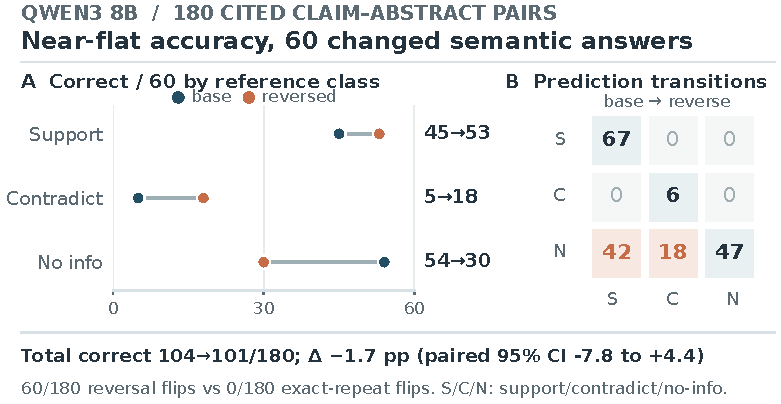
\includegraphics[width=.99\linewidth]{figures/fig_scifact3_compact.pdf}
\caption{Qwen's hidden cancellation on the balanced three-class SciFact diagnostic. Left: reference-correct counts by class on the same 60 pairs; right: complete 3$\times$3 semantic prediction transitions across all 180 pairs (S/C/N denote SUPPORT/CONTRADICT/NOINFO). Overall correctness changes little despite 60 label switches, all away from baseline NOINFO predictions. The paired interval uses 10,000 label-stratified claim/document-cluster resamples; exact-repeat switches were zero. NOINFO is restricted to an explicitly cited abstract without annotated evidence.}
\label{fig:scifact3}
\end{figure}

Title removal is a distinct sensitivity probe. For Laya English, it changes 60/180 labels and increases NOINFO reference-correct decisions from $20\to39/60$ ($+31.7$ points, $[+18.3,+45.0]$); the overall gain is $+10.6$ points ($[+3.9,+17.2]$). Other systems do not share a consistent gain (Table~\ref{tab:scifact3}). Removing a title also changes state serialization, while the frozen question still mentions that a title identifies the paper even when the field is absent; this is a visibility stressor, not proof of a lexical shortcut or a causal estimate of abstract reliance. The source's 138/71/130 candidate distribution was deliberately rebalanced, its annotations were not independently re-adjudicated, and no experiment here tests retrieval or full papers. The earlier two-choice positive-only SciFact slice overlaps this sample on only 28 SUPPORT and 55 CONTRADICT pairs; changed questions, label space and selection preclude a direct accuracy comparison. Source and input audits are detailed in Appendix~\ref{app:scifact3-audit} and the companion artifact.
